	\begin{figure}[!bhp]
	\centering
		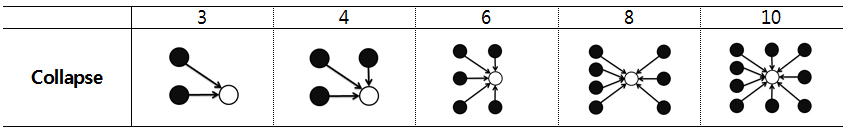
\includegraphics[height=50pt]{images/Topologies_Collapse}
		\caption{Bayesian Network Topology : Collapse}
	\end{figure}	

	% Collapse는 한 개의 자식 node에 여러 개의 부모 노드가 존재하는 형태이다.
	If one node has plurality of parent nodes, then this form called Collapse.

	\begin{figure}[!bhp]
	\centering
		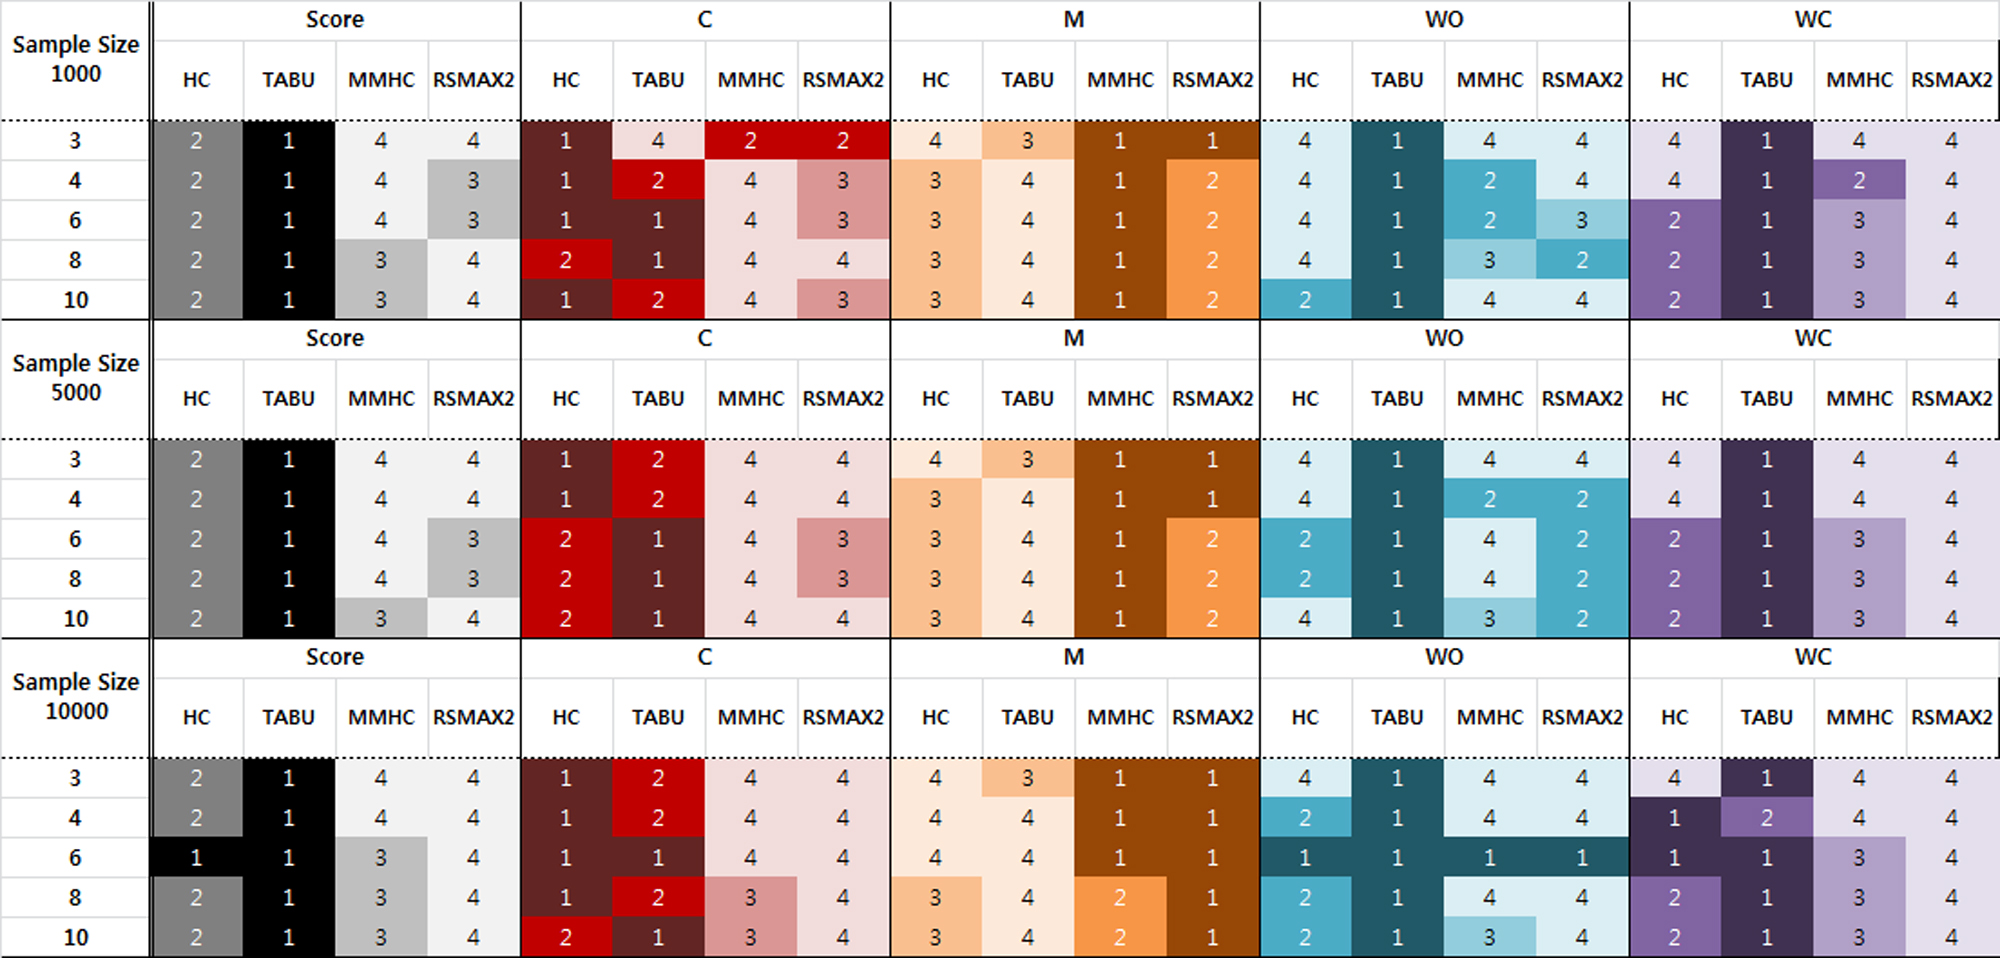
\includegraphics[height=155pt]{images/Result_Collapse}
		\caption{Summary for Comparison via Collapse}
	\end{figure}	

% Real data set을 이용할 때와 마찬가지로, score를 기준으로 하였을 때 TABU search 알고리즘, Hill-climbing 알고리즘 순으로 성능이 좋은 것으로 나타났다.
Like when using the Real data set, the TABU search is better than others according to score.

% 그러나 C의 개수는 TABU search와 Hill-climbing이 서로 경합을 벌였다. 오히려 TABU search의 경우 WO, WC의 개수가 많이 나타났다.
However, when compared by the number of C, TABU search and Hill-climbing has engaged in a conflict with each other. Rather the case of TABU search has a lot of WO and WC.

% Hill-climbing의 경우 TABU search만큼은 아니지만, node의 개수가 많아질수록, sample size가 커질수록 WO의 개수가 많아지는 현상이 나타났다.
Not as much as TABU search case of Hill-climbing, as more the number of nodes, and as much sample size, appeared that the number WO is larger.

% MMHC는 sample size가 커질수록 missing이 줄어드는 반면, RSMAX2는 오히려 늘어나는 현상이 나타났다.
While sample size increases, then M is decreasing when using MMHC, but M is increasing when using RSMAX2.
	
	\begin{figure}[p]
	\centering
		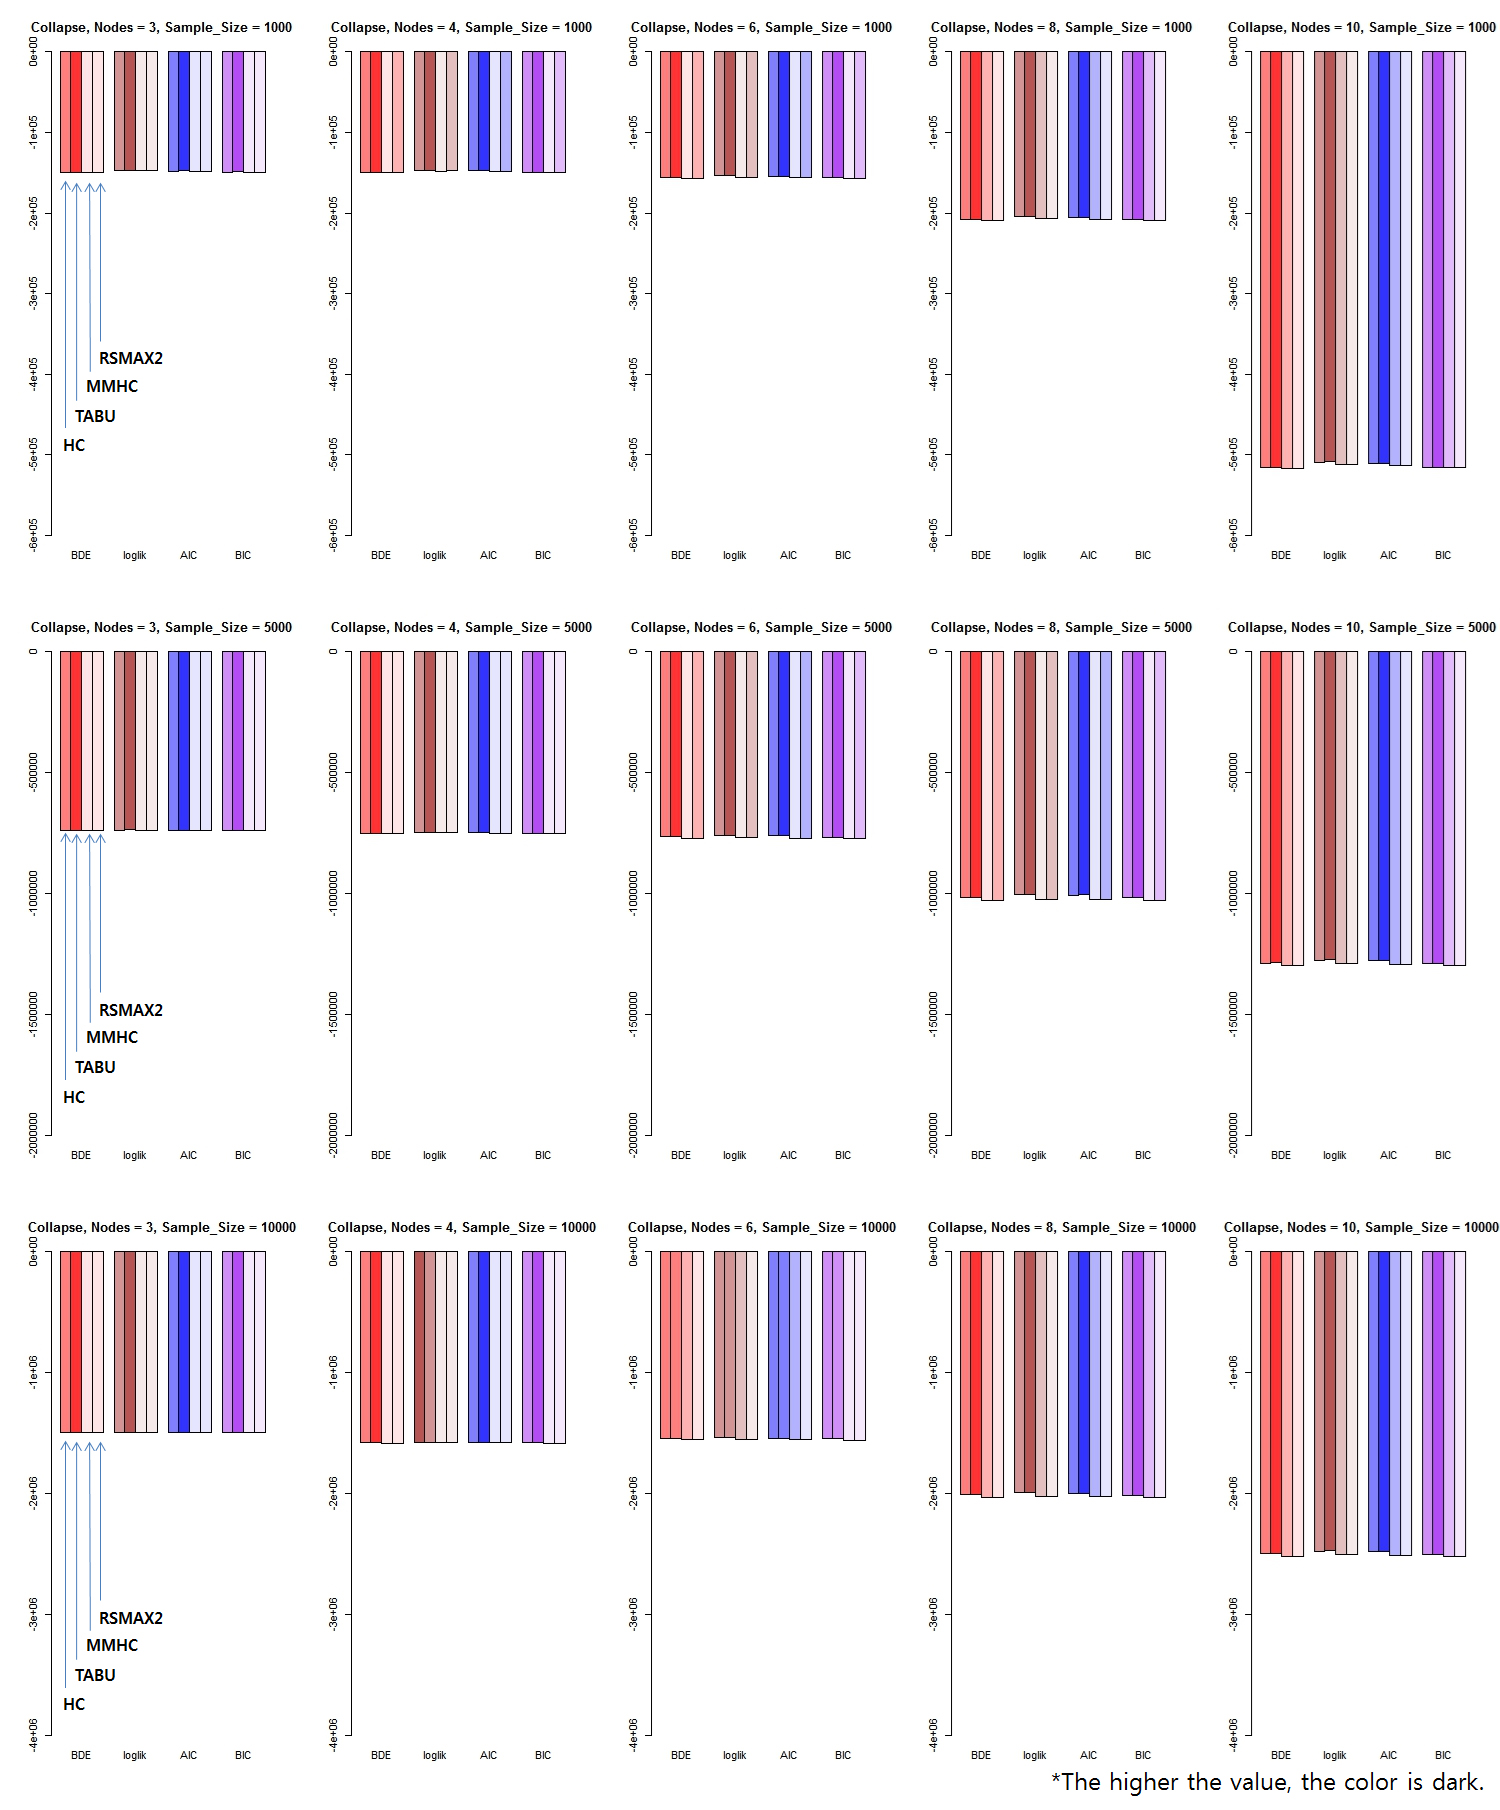
\includegraphics[height=500pt]{images/01_Collapse_Score}
		\caption{Comparison of scores via Collapse}
	\end{figure}	

	\begin{figure}[p]
	\centering
		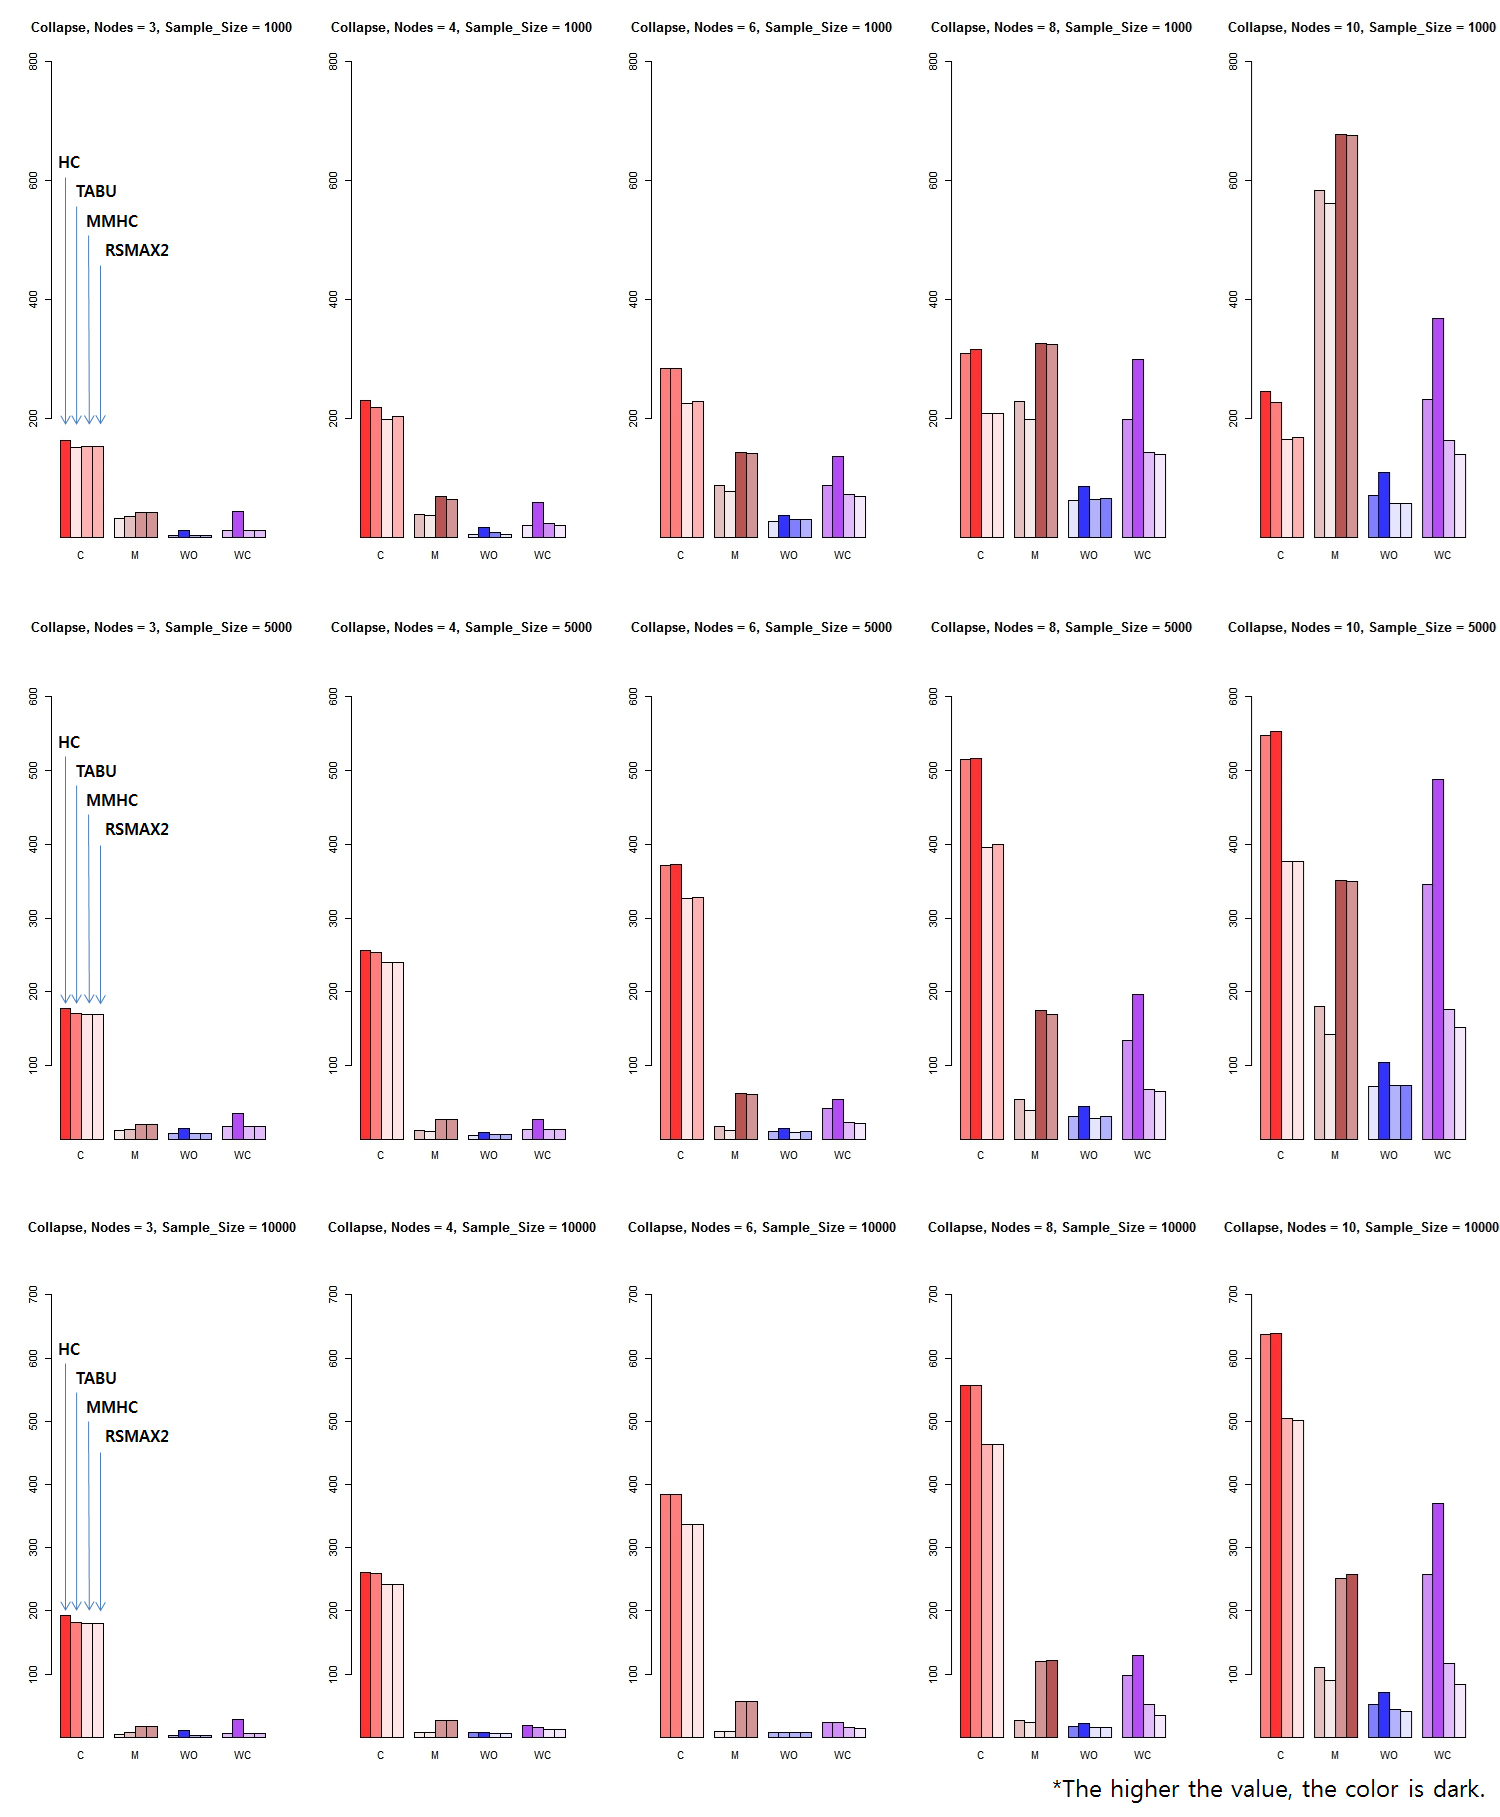
\includegraphics[height=500pt]{images/01_Collapse_Arcs}
		\caption{Comparison of correct arcs via Collapse}
	\end{figure}	

\newpage{}

